\documentclass{article}

\usepackage[font=small,labelfont=small]{caption}
\usepackage{subcaption}
\usepackage{float}
\usepackage{bm}
\usepackage{titlesec}
\usepackage{fancyhdr}
\usepackage{hyperref}
\usepackage[super,comma,compress]{natbib}
\usepackage{siunitx}
\usepackage{setspace}
\usepackage{helvet}
\bibliographystyle{unsrt}

\titleformat*{\section}{\normalsize\bfseries}
\titleformat*{\subsection}{\smallsize\bfseries}

\pagestyle{fancy}
\fancyhf{}
\rhead{\textit{\nouppercase{\leftmark}}}
\lhead{\textit{Argo Canada}}
\rfoot{\thepage}
\pagenumbering{arabic}
    

\title{DMQC Report on Dissolved Oxygen}
\author{Christopher Gordon, DMQC Operator}
\date{\today}

\begin{document}
\maketitle
\clearpage
\section{Float 4900494}

Gain (WOA): $0.995 \pm 0.020$
SAGE Gain: $1.035 \pm 0.025$

\begin{itemize}
	\item 0 flags should perhaps still be resolved, but assume visual QC is sufficient
	\item Removed one anomalous point that had very high O2sat
\end{itemize}


\begin{figure}[H]
	\centering
	\includegraphics[width=0.8\textwidth]{/Users/GordonC/Documents/projects/meds-dmqc/figures/4900494/gainplot.png}
	\caption{}
\end{figure}


\begin{figure}[H]
	\centering
	\includegraphics[width=0.8\textwidth]{/Users/GordonC/Documents/projects/meds-dmqc/figures/4900494/gainprofiles.png}
	\caption{}
\end{figure}


\begin{figure}[H]
	\centering
	\includegraphics[width=0.8\textwidth]{/Users/GordonC/Documents/projects/meds-dmqc/figures/4900494/qcprofiles.png}
	\caption{}
\end{figure}


\begin{figure}[H]
	\centering
	\includegraphics[width=0.8\textwidth]{/Users/GordonC/Documents/projects/meds-dmqc/figures/4900494/qcprofiles_cleaned.png}
	\caption{}
\end{figure}

\section{Float 4900497}

Gain (WOA): $1.031 \pm 0.024$

\begin{itemize}
	\item Various errors in FileChecker of forbidden attribute ``\_ChunkSize'', but I can't find that when I load the actual netcdf file
	\item 0 flags should perhaps still be resolved, but assume visual QC is sufficient
	\item In-air DOXY is in BRtraj file, but as DOXY, not PPOX\_DOXY. Upon further inspection BRtraj DOXY are all FillValues, so no in-air gain calculated.
\end{itemize}


\begin{figure}[H]
	\centering
	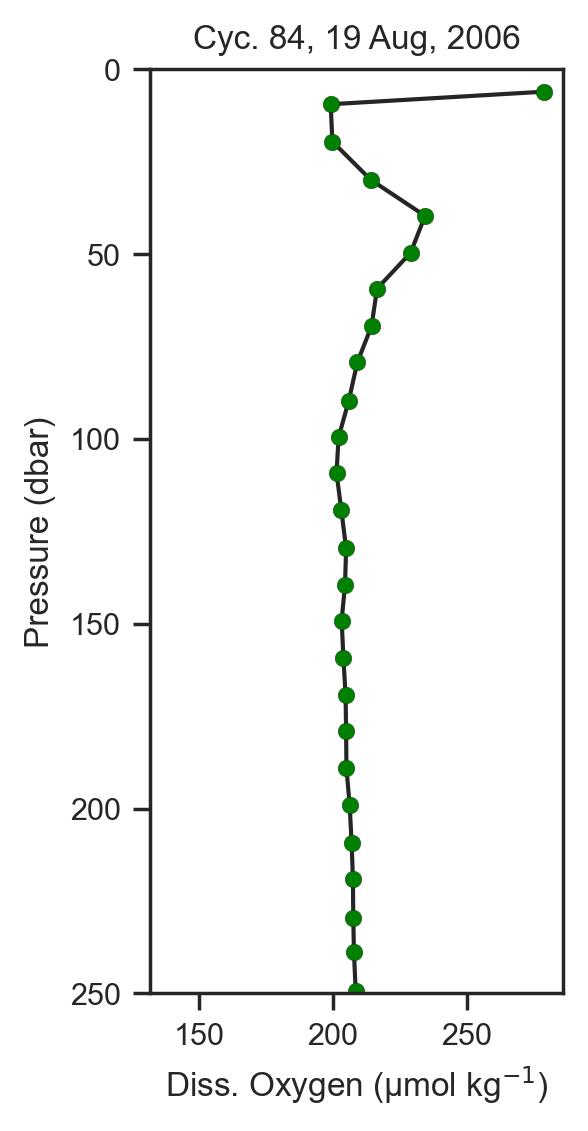
\includegraphics[width=0.8\textwidth]{/Users/GordonC/Documents/projects/meds-dmqc/figures/4900497/anom_profile.png}
	\caption{}
\end{figure}


\begin{figure}[H]
	\centering
	\includegraphics[width=0.8\textwidth]{/Users/GordonC/Documents/projects/meds-dmqc/figures/4900497/gainplot.png}
	\caption{}
\end{figure}


\begin{figure}[H]
	\centering
	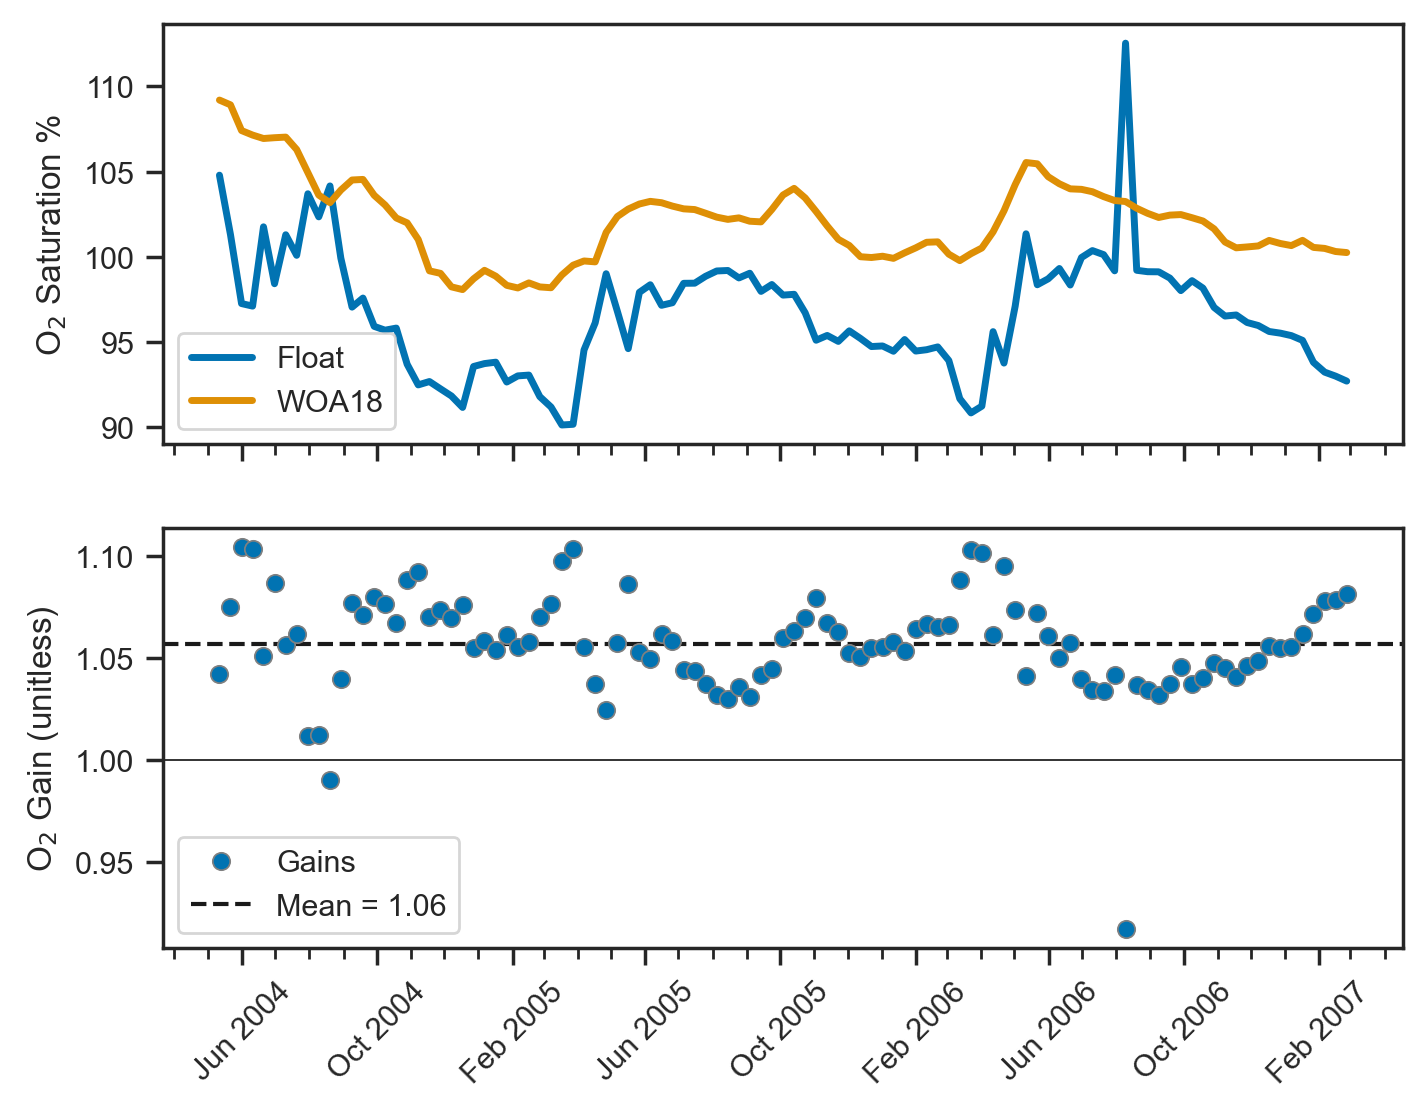
\includegraphics[width=0.8\textwidth]{/Users/GordonC/Documents/projects/meds-dmqc/figures/4900497/gainplot_20210621.png}
	\caption{}
\end{figure}


\begin{figure}[H]
	\centering
	\includegraphics[width=0.8\textwidth]{/Users/GordonC/Documents/projects/meds-dmqc/figures/4900497/gainprofiles.png}
	\caption{}
\end{figure}


\begin{figure}[H]
	\centering
	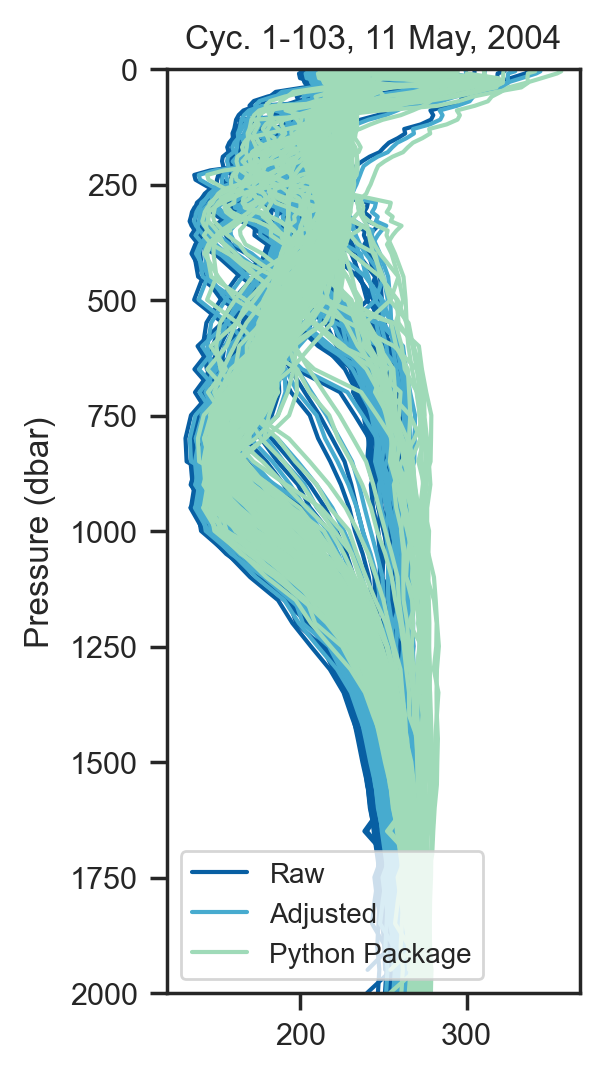
\includegraphics[width=0.8\textwidth]{/Users/GordonC/Documents/projects/meds-dmqc/figures/4900497/gainprofiles_20210621.png}
	\caption{}
\end{figure}


\begin{figure}[H]
	\centering
	\includegraphics[width=0.8\textwidth]{/Users/GordonC/Documents/projects/meds-dmqc/figures/4900497/new_gainplot.png}
	\caption{}
\end{figure}


\begin{figure}[H]
	\centering
	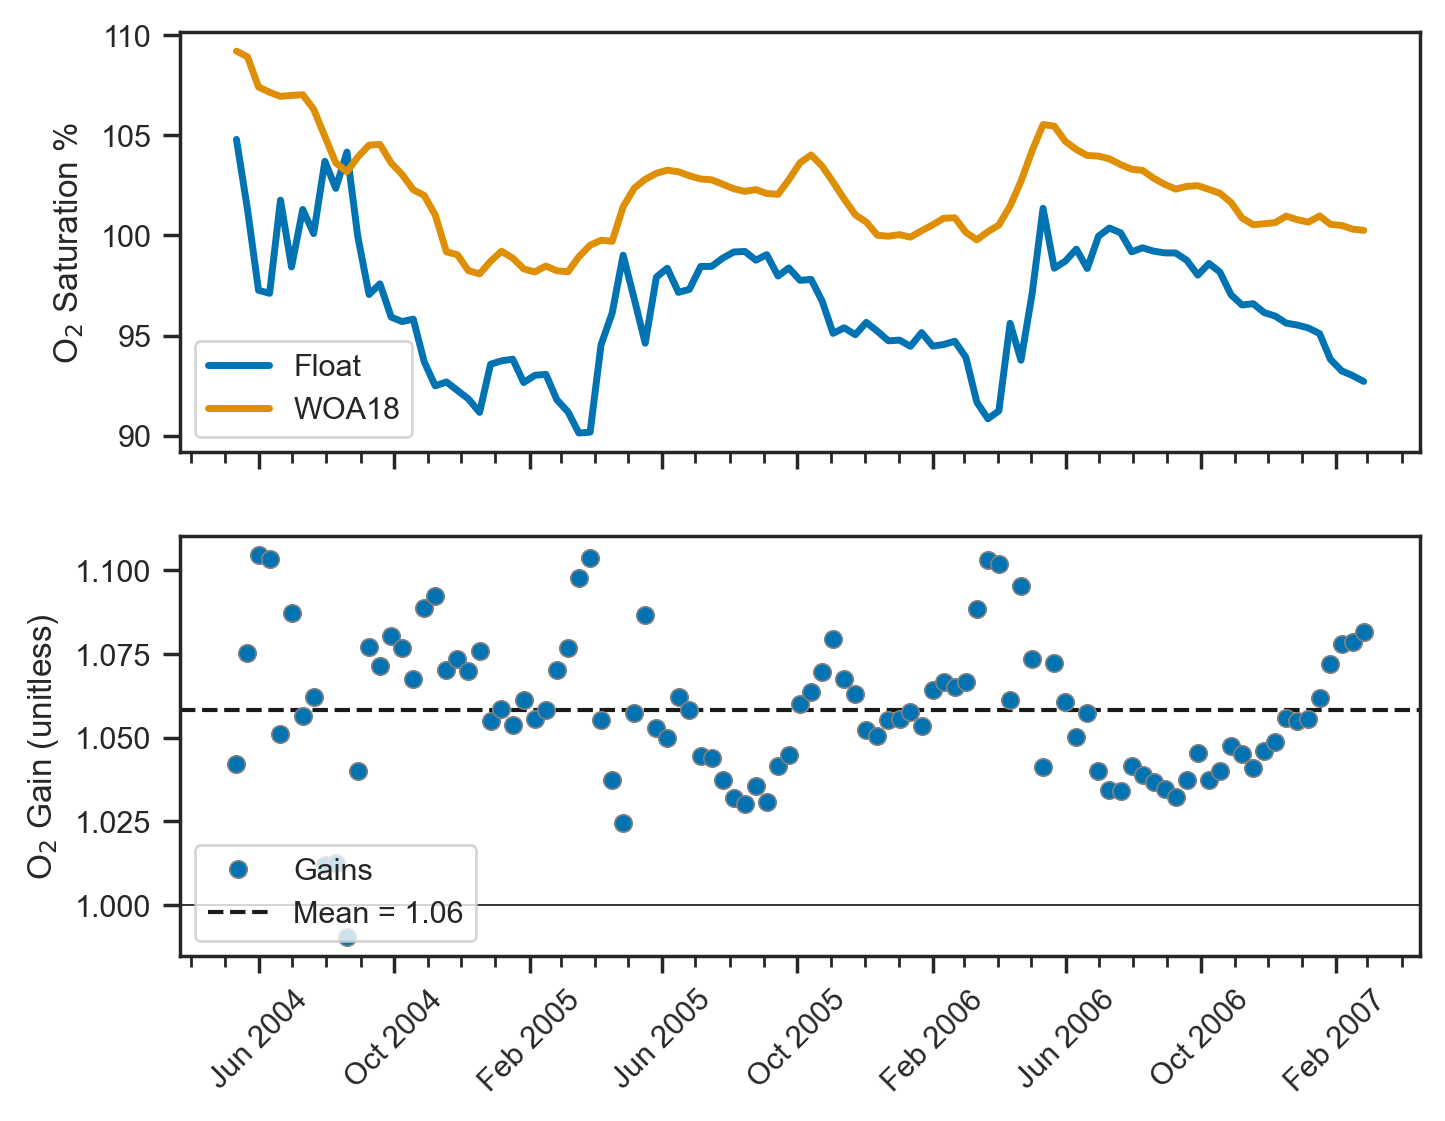
\includegraphics[width=0.8\textwidth]{/Users/GordonC/Documents/projects/meds-dmqc/figures/4900497/new_gainplot_20210621.png}
	\caption{}
\end{figure}


\begin{figure}[H]
	\centering
	\includegraphics[width=0.8\textwidth]{/Users/GordonC/Documents/projects/meds-dmqc/figures/4900497/new_new_gainplot.png}
	\caption{}
\end{figure}


\begin{figure}[H]
	\centering
	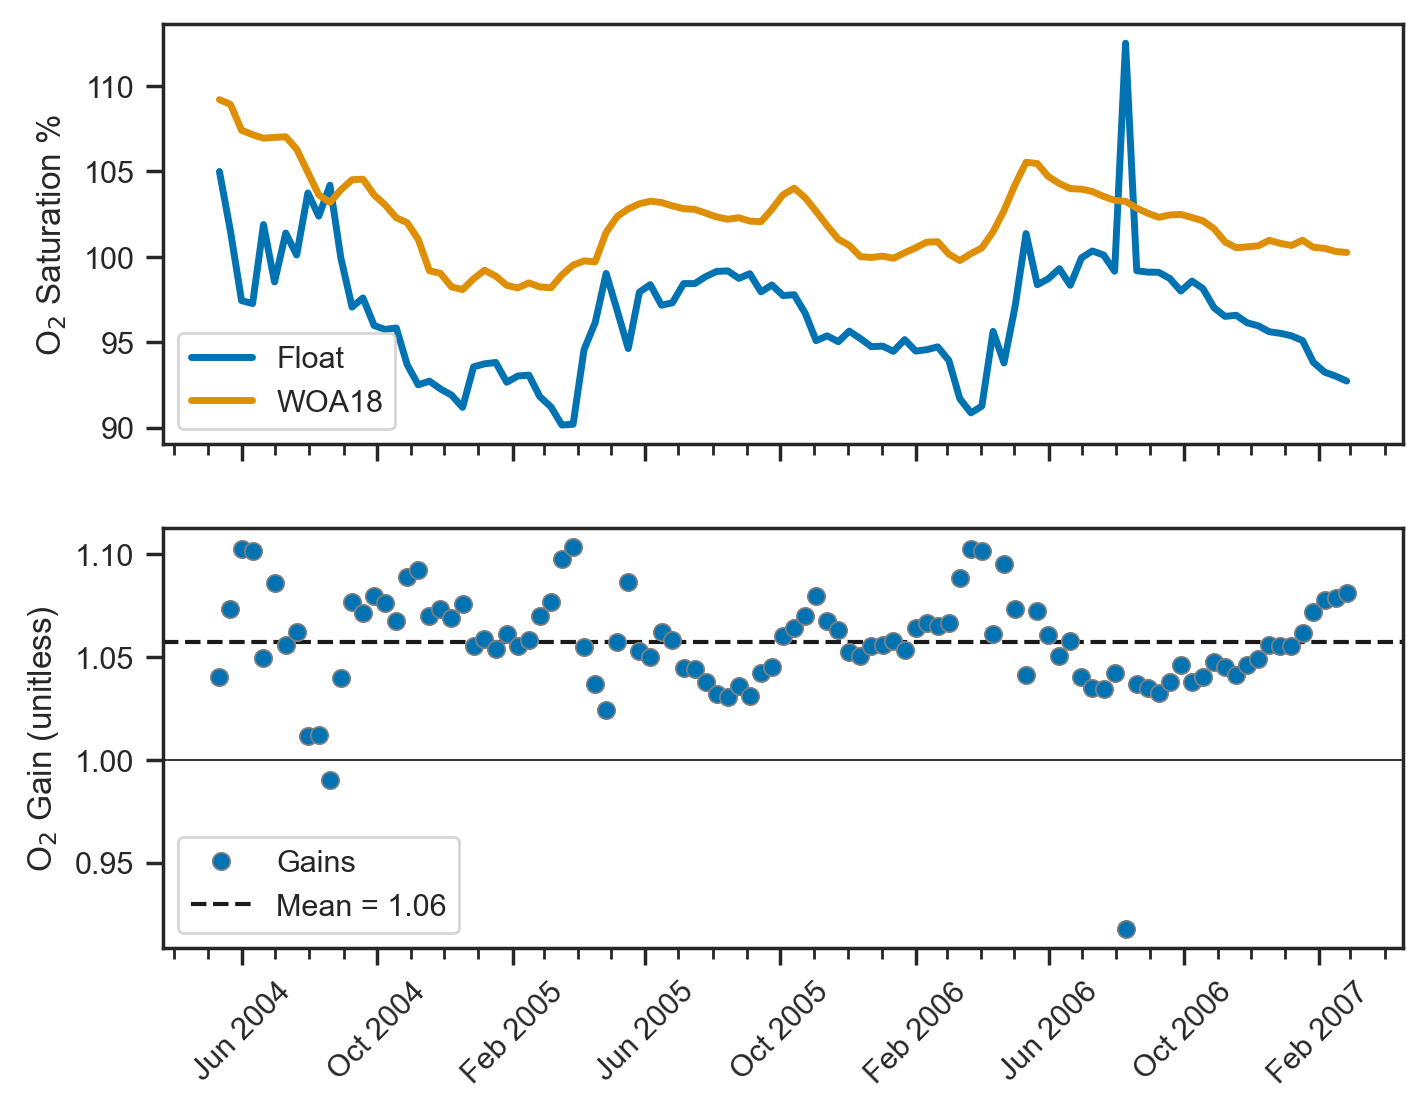
\includegraphics[width=0.8\textwidth]{/Users/GordonC/Documents/projects/meds-dmqc/figures/4900497/new_new_gainplot_20210621.png}
	\caption{}
\end{figure}


\begin{figure}[H]
	\centering
	\includegraphics[width=0.8\textwidth]{/Users/GordonC/Documents/projects/meds-dmqc/figures/4900497/new_sage_comparison.png}
	\caption{}
\end{figure}


\begin{figure}[H]
	\centering
	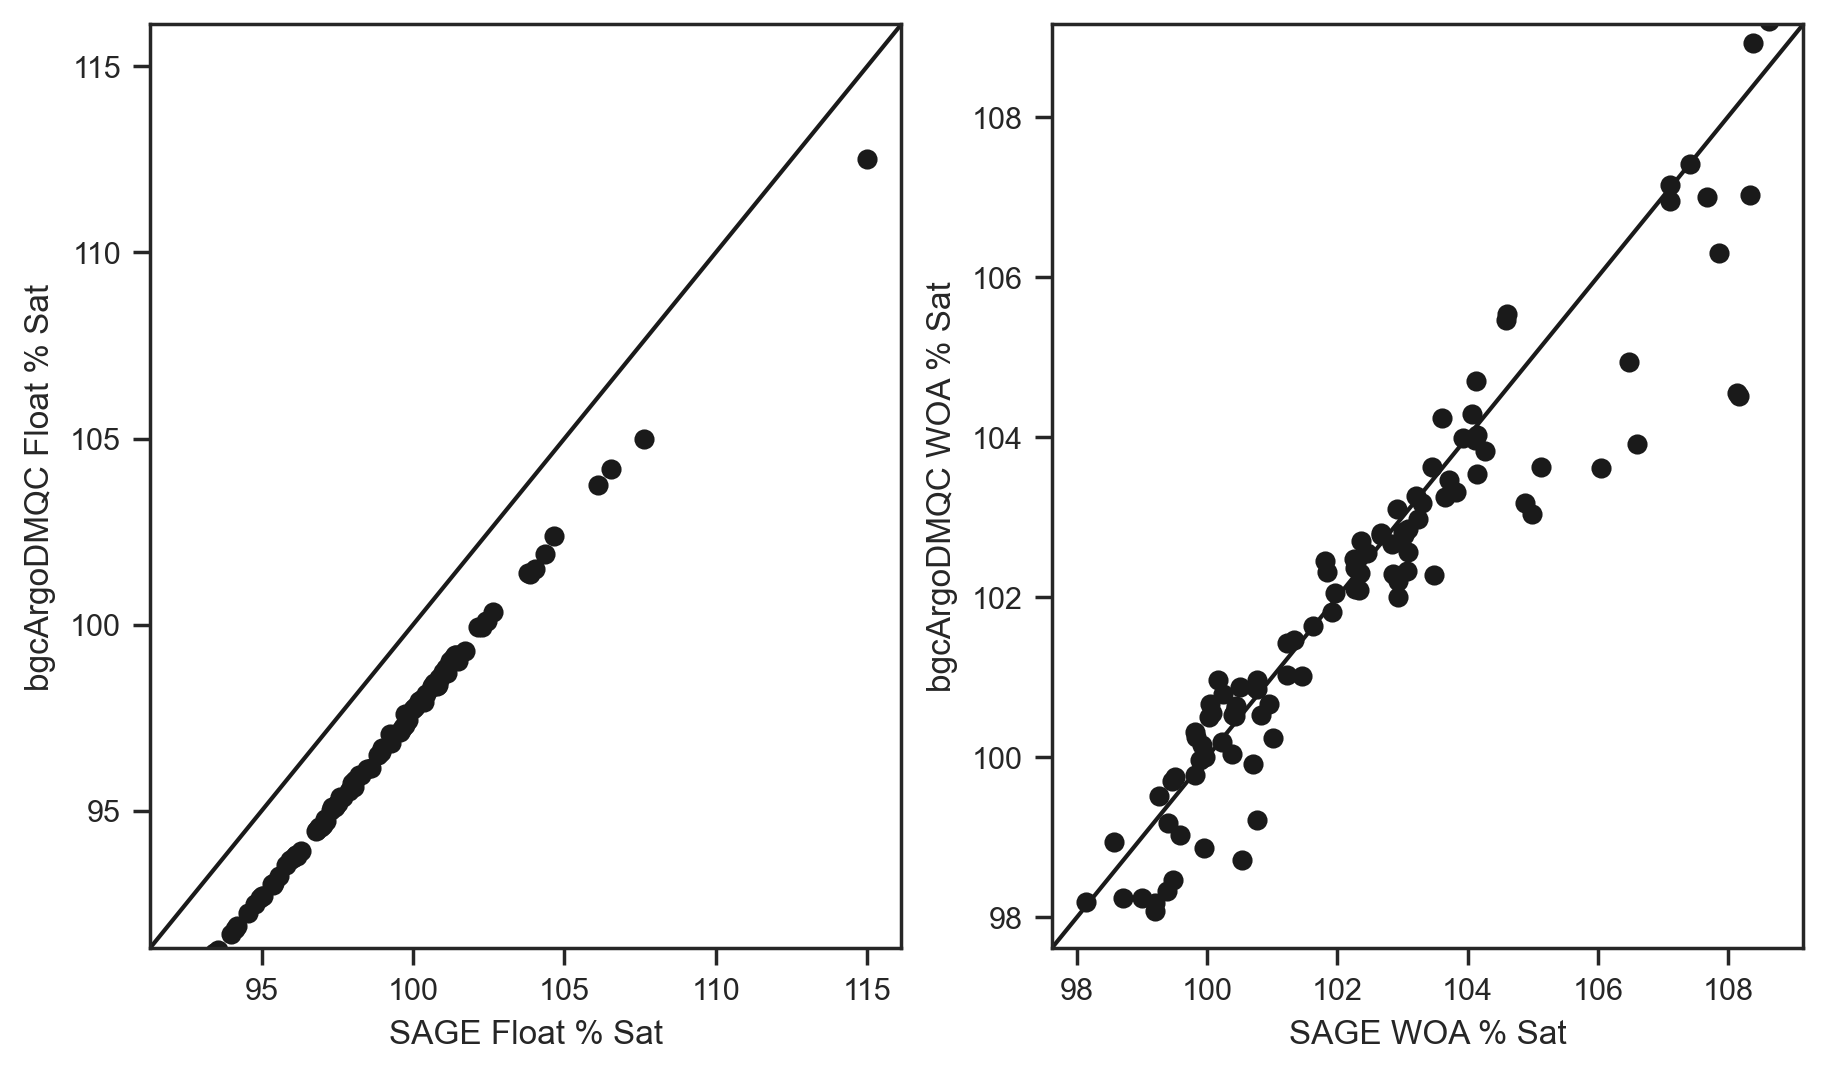
\includegraphics[width=0.8\textwidth]{/Users/GordonC/Documents/projects/meds-dmqc/figures/4900497/new_sage_comparison_20210621.png}
	\caption{}
\end{figure}


\begin{figure}[H]
	\centering
	\includegraphics[width=0.8\textwidth]{/Users/GordonC/Documents/projects/meds-dmqc/figures/4900497/qcprofiles.png}
	\caption{}
\end{figure}


\begin{figure}[H]
	\centering
	\includegraphics[width=0.8\textwidth]{/Users/GordonC/Documents/projects/meds-dmqc/figures/4900497/qcprofiles_cleaned.png}
	\caption{}
\end{figure}


\begin{figure}[H]
	\centering
	\includegraphics[width=0.8\textwidth]{/Users/GordonC/Documents/projects/meds-dmqc/figures/4900497/sage_comparison.png}
	\caption{}
\end{figure}


\begin{figure}[H]
	\centering
	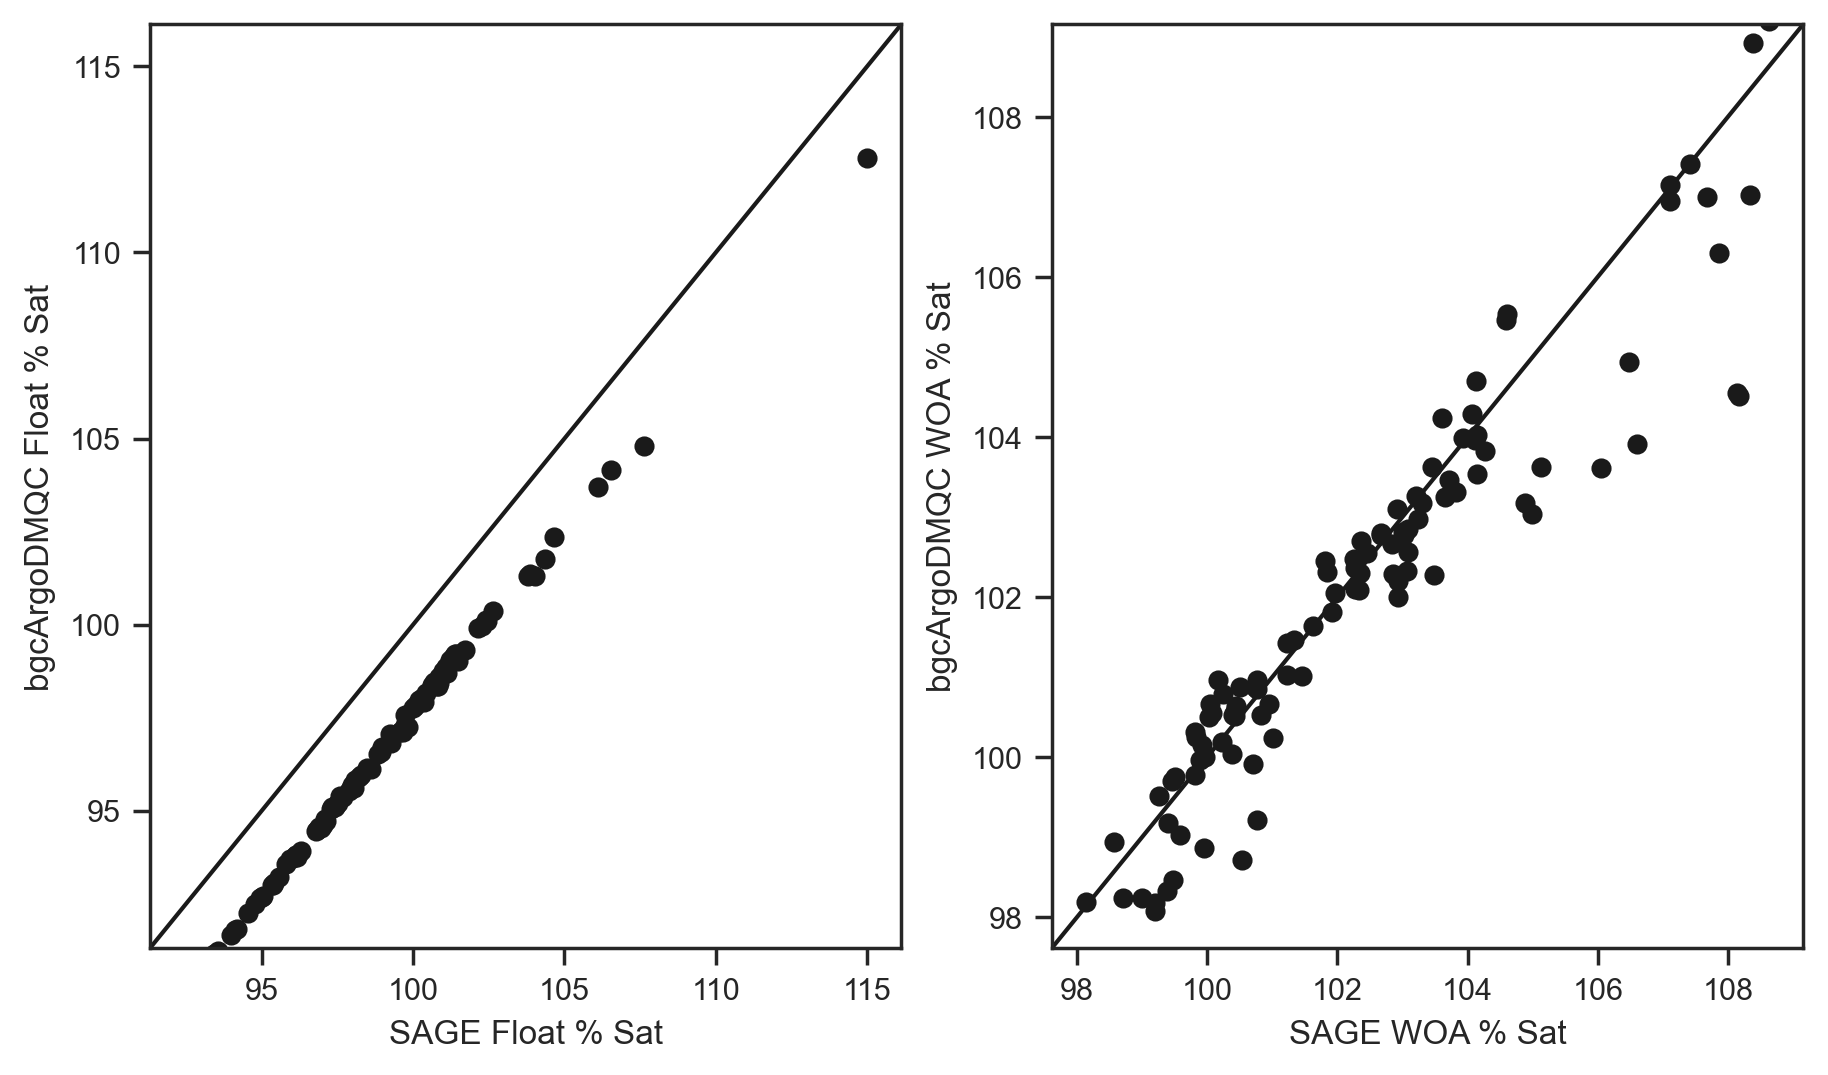
\includegraphics[width=0.8\textwidth]{/Users/GordonC/Documents/projects/meds-dmqc/figures/4900497/sage_comparison_20210621.png}
	\caption{}
\end{figure}


\begin{figure}[H]
	\centering
	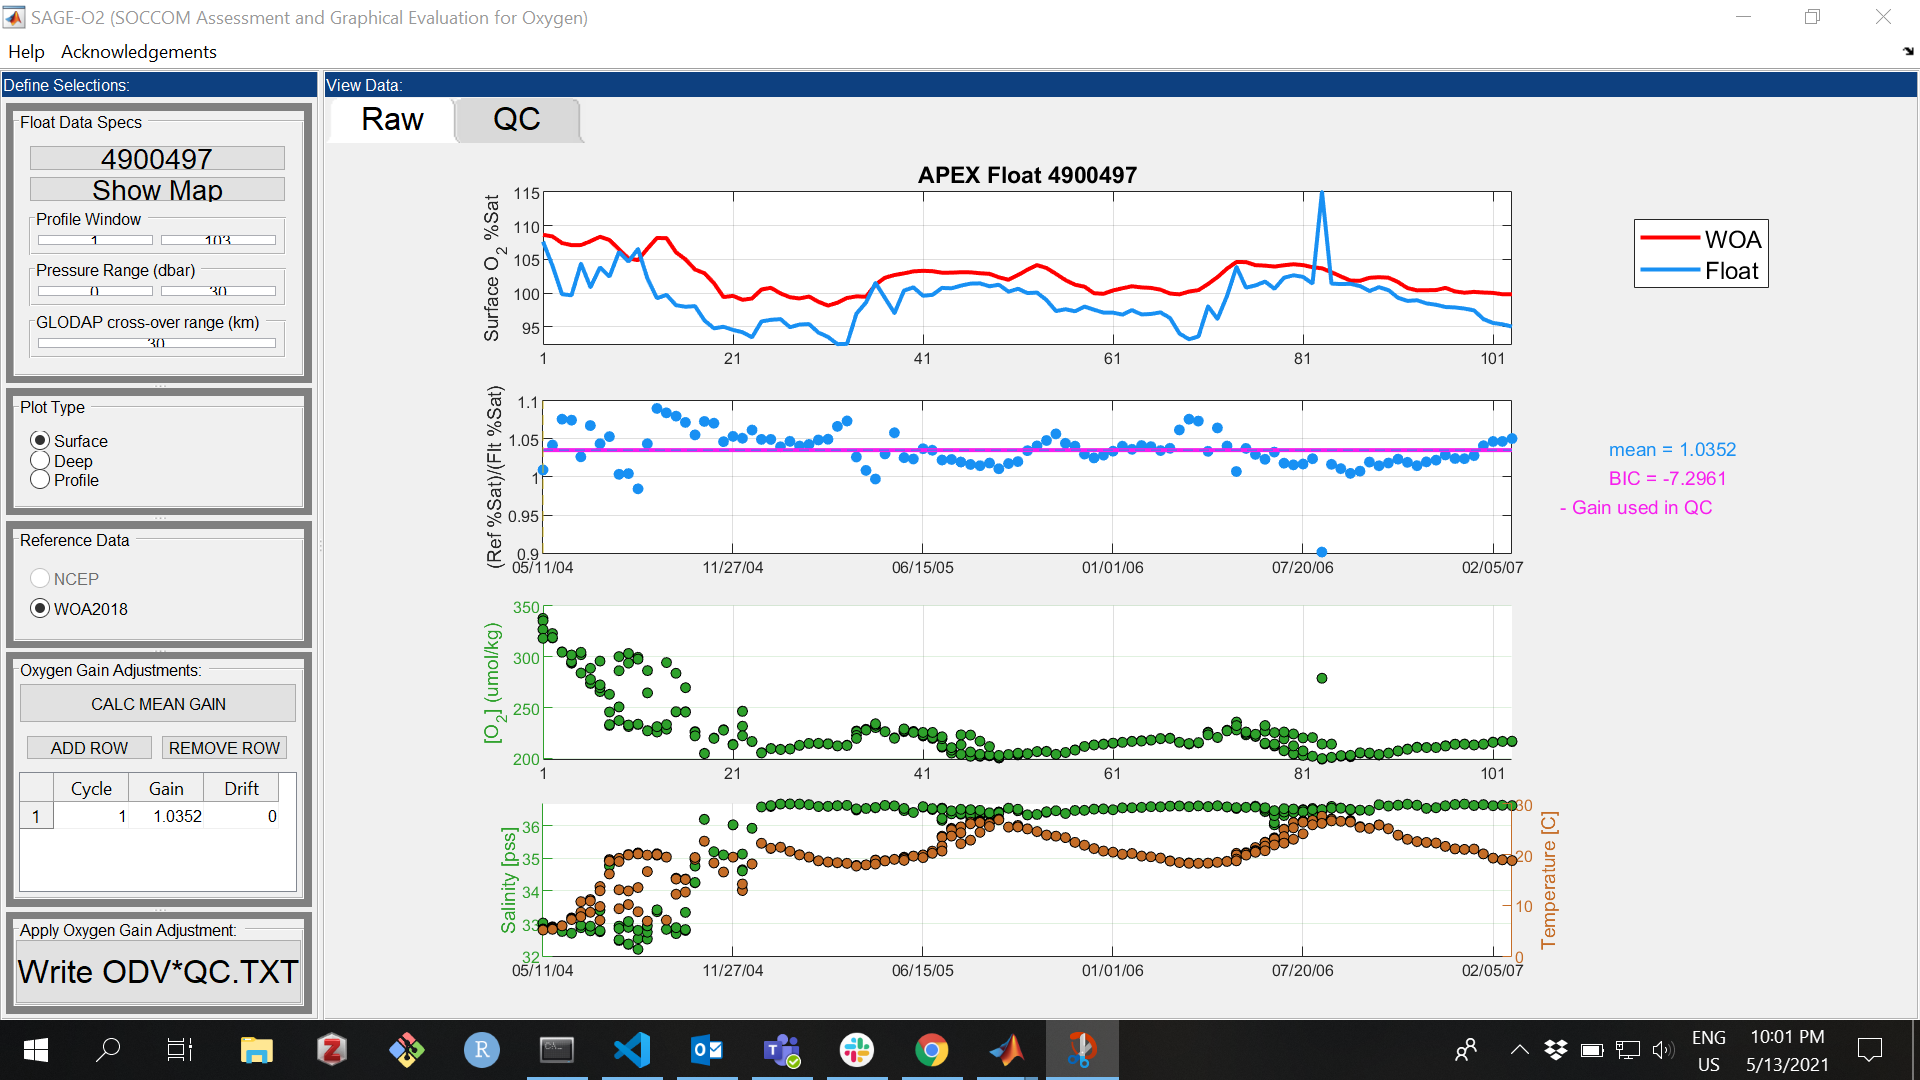
\includegraphics[width=0.8\textwidth]{/Users/GordonC/Documents/projects/meds-dmqc/figures/4900497/SAGE_screenshot.png}
	\caption{}
\end{figure}

\section{Float 4900523}

Gain (WOA): $1.045 \pm 0.015$
SAGE Gain: $1.043 \pm 0.025$

\begin{itemize}
	\item Upon inspection of profiles, there are one point for salinity and one for oxygen that seem to be anomalous
	\begin{itemize}
		\item interpolated salinity point, cycle 112, P < 94dbar and S > 33.80psu
		\item oxygen point, the same as the salinity point where O2 < 69mmol m$^{-3}$
	\end{itemize}
	\item There is one point with a significant divergence from SAGE, but I do not believe that is in error, but rather a point that should be flagged as bad, and SAGE did not. Therefore in SAGE the point has a much higher O2Sat than in the python package.
\end{itemize}


\begin{figure}[H]
	\centering
	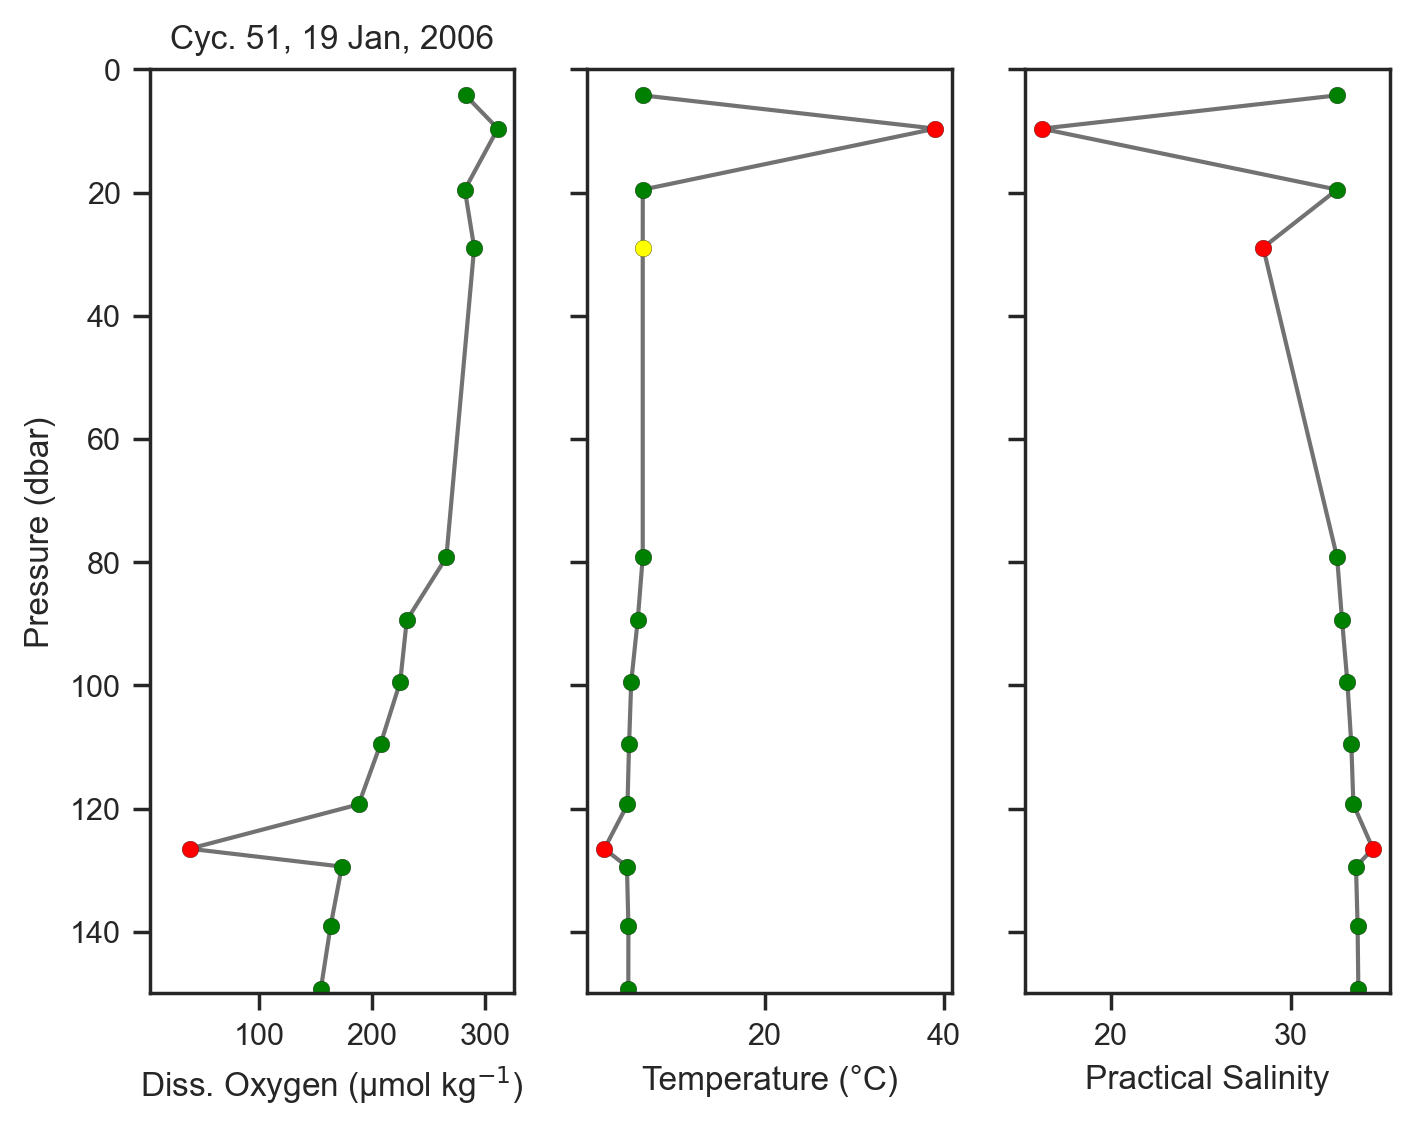
\includegraphics[width=0.8\textwidth]{/Users/GordonC/Documents/projects/meds-dmqc/figures/4900523/anom_profile_g=0.82.png}
	\caption{}
\end{figure}


\begin{figure}[H]
	\centering
	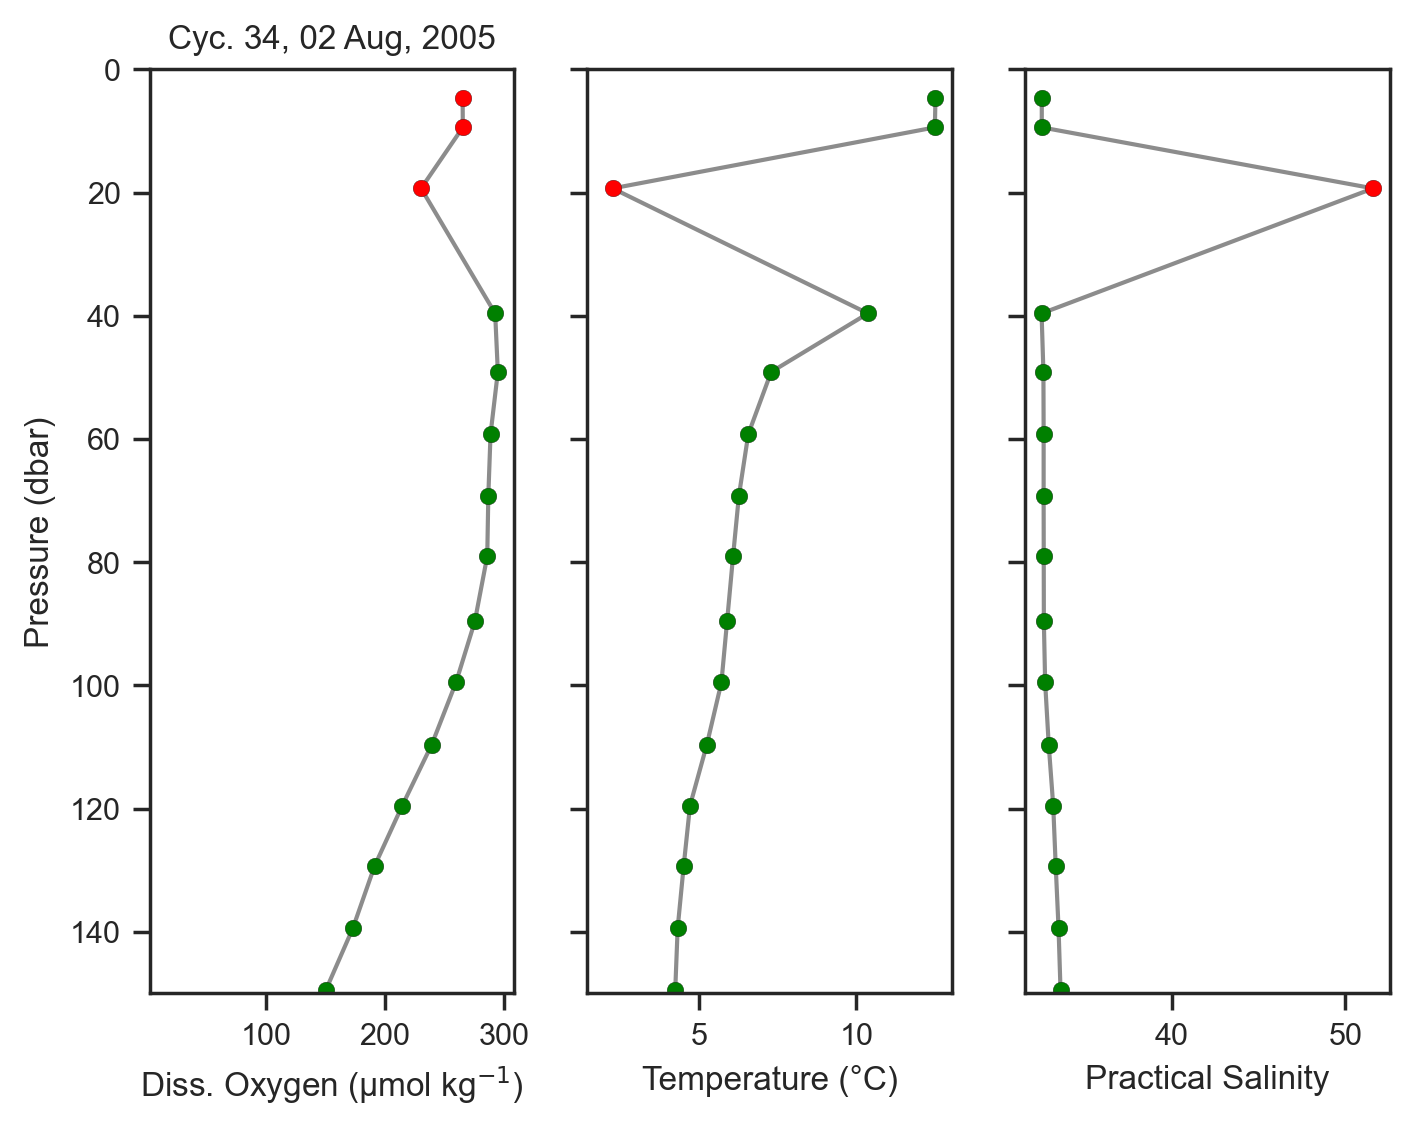
\includegraphics[width=0.8\textwidth]{/Users/GordonC/Documents/projects/meds-dmqc/figures/4900523/anom_profile_g=1.12.png}
	\caption{}
\end{figure}


\begin{figure}[H]
	\centering
	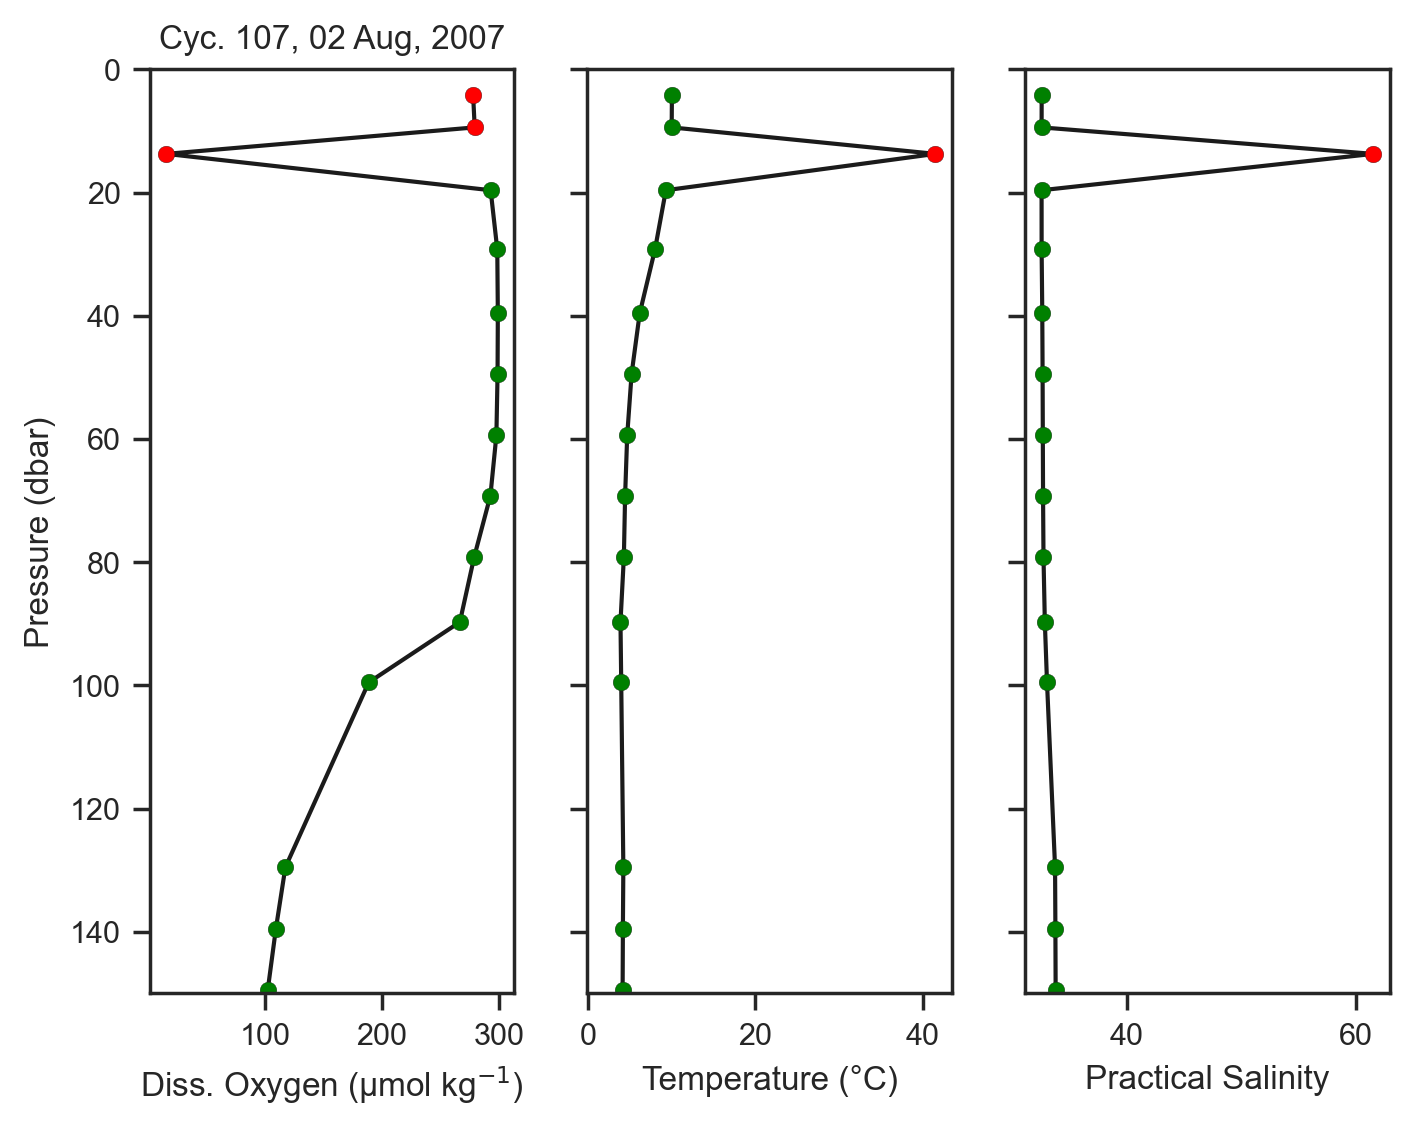
\includegraphics[width=0.8\textwidth]{/Users/GordonC/Documents/projects/meds-dmqc/figures/4900523/anom_profile_g=1.33.png}
	\caption{}
\end{figure}


\begin{figure}[H]
	\centering
	\includegraphics[width=0.8\textwidth]{/Users/GordonC/Documents/projects/meds-dmqc/figures/4900523/gainplot.png}
	\caption{}
\end{figure}


\begin{figure}[H]
	\centering
	\includegraphics[width=0.8\textwidth]{/Users/GordonC/Documents/projects/meds-dmqc/figures/4900523/gainprofiles.png}
	\caption{}
\end{figure}


\begin{figure}[H]
	\centering
	\includegraphics[width=0.8\textwidth]{/Users/GordonC/Documents/projects/meds-dmqc/figures/4900523/new_gainplot.png}
	\caption{}
\end{figure}


\begin{figure}[H]
	\centering
	\includegraphics[width=0.8\textwidth]{/Users/GordonC/Documents/projects/meds-dmqc/figures/4900523/qcprofiles.png}
	\caption{}
\end{figure}


\begin{figure}[H]
	\centering
	\includegraphics[width=0.8\textwidth]{/Users/GordonC/Documents/projects/meds-dmqc/figures/4900523/qcprofiles_cleaned.png}
	\caption{}
\end{figure}


\begin{figure}[H]
	\centering
	\includegraphics[width=0.8\textwidth]{/Users/GordonC/Documents/projects/meds-dmqc/figures/4900523/sage_comparison.png}
	\caption{}
\end{figure}

\section{Float 4900524}

Gain (WOA): $1.052 \pm 0.018$

\begin{itemize}
	\item Only 6 cycles, but ready to go.
\end{itemize}


\begin{figure}[H]
	\centering
	\includegraphics[width=0.8\textwidth]{/Users/GordonC/Documents/projects/meds-dmqc/figures/4900524/gainplot.png}
	\caption{}
\end{figure}


\begin{figure}[H]
	\centering
	\includegraphics[width=0.8\textwidth]{/Users/GordonC/Documents/projects/meds-dmqc/figures/4900524/gainprofiles.png}
	\caption{}
\end{figure}


\begin{figure}[H]
	\centering
	\includegraphics[width=0.8\textwidth]{/Users/GordonC/Documents/projects/meds-dmqc/figures/4900524/qcprofiles.png}
	\caption{}
\end{figure}


\begin{figure}[H]
	\centering
	\includegraphics[width=0.8\textwidth]{/Users/GordonC/Documents/projects/meds-dmqc/figures/4900524/qcprofiles_cleaned.png}
	\caption{}
\end{figure}

\section{Float 4900627}

Gain (WOA): $1.004 \pm 0.024$
SAGE Gain: $1.006 \pm 0.024$

\begin{itemize}
	\item DOXY exists in Brtraj file but is all FillValues.
\end{itemize}


\begin{figure}[H]
	\centering
	\includegraphics[width=0.8\textwidth]{/Users/GordonC/Documents/projects/meds-dmqc/figures/4900627/gainplot.png}
	\caption{}
\end{figure}


\begin{figure}[H]
	\centering
	\includegraphics[width=0.8\textwidth]{/Users/GordonC/Documents/projects/meds-dmqc/figures/4900627/gainprofiles.png}
	\caption{}
\end{figure}


\begin{figure}[H]
	\centering
	\includegraphics[width=0.8\textwidth]{/Users/GordonC/Documents/projects/meds-dmqc/figures/4900627/new_gainplot.png}
	\caption{}
\end{figure}


\begin{figure}[H]
	\centering
	\includegraphics[width=0.8\textwidth]{/Users/GordonC/Documents/projects/meds-dmqc/figures/4900627/new_new_gainplot.png}
	\caption{}
\end{figure}


\begin{figure}[H]
	\centering
	\includegraphics[width=0.8\textwidth]{/Users/GordonC/Documents/projects/meds-dmqc/figures/4900627/new_sage_comparison.png}
	\caption{}
\end{figure}


\begin{figure}[H]
	\centering
	\includegraphics[width=0.8\textwidth]{/Users/GordonC/Documents/projects/meds-dmqc/figures/4900627/qcprofiles.png}
	\caption{}
\end{figure}


\begin{figure}[H]
	\centering
	\includegraphics[width=0.8\textwidth]{/Users/GordonC/Documents/projects/meds-dmqc/figures/4900627/qcprofiles_cleaned.png}
	\caption{}
\end{figure}


\begin{figure}[H]
	\centering
	\includegraphics[width=0.8\textwidth]{/Users/GordonC/Documents/projects/meds-dmqc/figures/4900627/sage_comparison.png}
	\caption{}
\end{figure}

\section{Float 4900637}

Gain (WOA): $0.989 \pm 0.013$

\begin{itemize}
	\item The last 3 profiles of salinity are flagged as 3, and then for the remaining lifetime of the float are 4. There are two issues here
	\begin{itemize}
		\item the salinity that is flagged as 3 I believe should be flagged as 4, as it is quite low (about 15) and throws off density enough that the O2 saturation percent is off significantly where salinity is flagged 4, oxygen should be flagged 3, but is currently flagged 1
	\end{itemize}
	\item Since salinity is 4 after July 2007, there are only valid O2sat values for the first half of the floats life. The O2sat values where PSAL\_QC = 3 were excluded from the gain calculation.
\end{itemize}


\begin{figure}[H]
	\centering
	\includegraphics[width=0.8\textwidth]{/Users/GordonC/Documents/projects/meds-dmqc/figures/4900637/gainplot.png}
	\caption{}
\end{figure}


\begin{figure}[H]
	\centering
	\includegraphics[width=0.8\textwidth]{/Users/GordonC/Documents/projects/meds-dmqc/figures/4900637/gainprofiles.png}
	\caption{}
\end{figure}


\begin{figure}[H]
	\centering
	\includegraphics[width=0.8\textwidth]{/Users/GordonC/Documents/projects/meds-dmqc/figures/4900637/new_gainplot.png}
	\caption{}
\end{figure}


\begin{figure}[H]
	\centering
	\includegraphics[width=0.8\textwidth]{/Users/GordonC/Documents/projects/meds-dmqc/figures/4900637/qcprofiles.png}
	\caption{}
\end{figure}


\begin{figure}[H]
	\centering
	\includegraphics[width=0.8\textwidth]{/Users/GordonC/Documents/projects/meds-dmqc/figures/4900637/qcprofiles_cleaned.png}
	\caption{}
\end{figure}

\end{document}
